\section{Kết luận}
\subsection{Kết quả đạt được và điểm hạn chế}
Đối với đề tài này, ở giai đoạn đồ án chuyên ngành, chúng tôi đã đạt được một số kết quả nhất định.
Thứ nhất, chúng tôi đã hiện thực được không gian quản lý các dự án và các quy trình nghiệp vụ, cho phép người dùng chia sẻ không gian 
để mở rộng và cộng tác với nhiều thành viên khác trong hệ thống. Thứ hai, chúng tôi đã xây dựng được lý thuyết đánh giá chất lượng của quy
trình nghiệp vụ, cũng như lý thuyết về mức độ ưu tiên của quy trình nghiệp vụ trong một nhóm các quy trình trong Workspace. Đây là nền tảng
vững chắc để phát triển hệ thống trong giai đoạn luận văn.
\par
Tuy nhiên, đồ án chuyên ngành còn một số hạn chế. Thứ nhất, chúng tôi chưa khắc phục triệt để những lỗi về giao diện người dùng còn tồn
đọng từ đề tài trước, cũng như một số lỗi giao diện phát sinh ở đề tài này. Thứ hai, chúng tôi chưa hiện thực tính năng cá nhân hoá
Workspace. Thứ ba, hệ thống thông báo chỉ mới có hai loại thông báo cơ bản là thông báo về lời mời tham gia Workspace và thông báo trạng thái
của yêu cầu thay đổi quyền hạn của bản thân người dùng trong Workspace, và chúng tôi cho rằng cần phải mở rộng hệ thống thông báo để
người dùng có thể nhận được thông báo về những hoạt động quan trọng khác trong Workspace cũng như trong hệ thống.

\subsection{Hướng phát triển cho giai đoạn luận văn}
Ở giai đoạn luận văn, chúng tôi sẽ tiếp tục phát triển hệ thống với những hướng phát triển sau:
\begin{itemize}
    \item Hoàn thiện tính năng thiết kế bảng khảo sát, chia sẻ và thu nhận kết quả khảo sát.
    \item Hoàn thiện chức năng đánh giá chất lượng của quy trình nghiệp vụ.
    \item Hiện thực chức năng trực quan hoá mức độ ưu tiên của quy trình nghiệp vụ.
    \item Hiện thực tính năng đề xuất bản thiết kế quy trình, giúp người dùng chọn lựa quy trình nghiệp vụ mẫu có sẵn phù hợp với nhu cầu của mình.
    \item Mở rộng hệ thống, hướng đến cho phép người dùng đóng góp, chia sẻ thiết kế, đánh giá của quy trình nghiệp vụ cho những người dùng khác trong hệ thống.
\end{itemize}

\subsection{Kế hoạch làm việc dự kiến cho giai đoạn luận văn}
Dựa vào những hướng phát triển đã đề ra, chúng tôi vạch ra kế hoạch làm việc dự kiến cho giai đoạn luận văn như sau:
\begin{figure}[H]
    \centering
    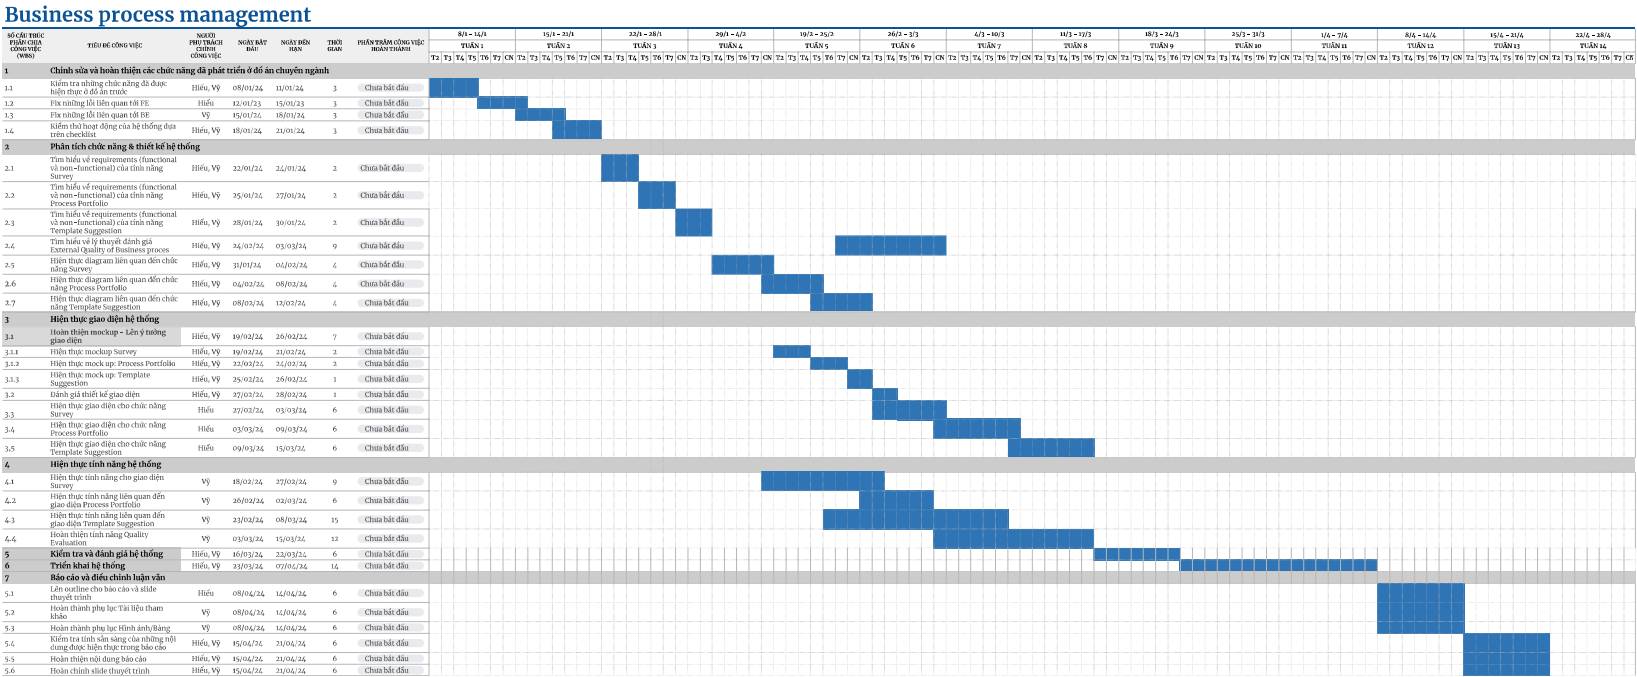
\includegraphics[width=\linewidth]{Content/Kết luận/images/graduteschedule.png}
    \vspace{0.5cm}
    \caption{Biểu đồ Gantt cho kế hoạch làm việc dự kiến cho giai đoạn luận văn}
    \label{fig:Biểu đồ Gantt cho kế hoạch làm việc dự kiến cho giai đoạn luận văn}
\end{figure}